\section{Response to Reviewer 9}
% \begin{bibunit}
\textbf{Reviewer 9—General comments—}\textit{%
This letter discusses an interesting topic about the number of future control inputs to transfer in the wireless networked control systems. However, this version is a little mess in notations, descriptions, resulting a challenge of readability. I believe a major improvement is necessary for publishing. The comments are as follows.}\\[2mm]
\textbf{Authors' response:} \textcolor{black}{We appreciate the Reviewer's feedback. In the revised version, we have carefully addressed the Reviewer's concerns and made necessary modifications.}\\[4mm]
%%%
\textbf{Reviewer 9–Comment 1—}\textit{%
Motivation is not enough, especially in the Sec. I—Introduction, it is not clearly for the contribution through comparing with the existing relevant research. 
Besides, authors underline that a practical hidden Markov jump linear system (HMJLS) model is one of the contributions of this letter. 
I wonder if it is the first time to propose it, or, you setup the model from a novel perspective. Description and analysis are necessary.}\\[2mm]
\textbf{Authors' response 1:} \textcolor{black}{We thank the Reviewer for the valuable comment. Due to the strict page limit of an L-CSS letter, we lack the space to provide an in-depth discussion of the state of the art, which is available in the references [1]–[5]. The relevance of the topic is thoroughly discussed there. This letter is motivated by two significant shortcomings of the previous relevant works, particularly [4] and [5]: the channel state information may be unavailable or imperfect, and transmitting future control inputs is a compelling alternative to sending only the current one, as outlined in the introduction. This letter addresses these two limitations of the previous research and significantly extends the results in [4]. The provided results greatly enhance the practical relevance of the wireless-channel-state-dependent control strategies by accounting for the channel state estimation with measurement noise and more advanced control strategies. The hidden Markov jump linear system (HMJLS) model of discrete-time linear stochastic systems with hybrid MDC and imperfect CSI is indeed introduced in this letter for the first time. Under perfect CSI and without future control inputs, this model reduces to the Markov jump linear system in [4]. This generalization presents several significant conceptual and technical challenges that are addressed throughout this letter. Unfortunately, the length constraint prevents us from including this clarification in the manuscript. We use all the available limited space to address the suggestion in the following comment about the sketch for the closed-loop system.}\\[4mm]
%%%
\textbf{Reviewer 9—Comment 2—}\textit{%
I suggest you to add a sketch for the closed-loop system, or the basic idea of the letter, for readability. Especially, a lot of components are considered in this letter, it is necessary to have a clear structure and highlight key points.}\\[2mm]
\textbf{Authors' response 2:} \textcolor{violet}{OK}\\[4mm]
%%%
\textbf{Reviewer 9—Comment 3—}\textit{%
If LQR is used as the feedback controller, if T is infinite, we can get the control gain K offline, there is no need to discuss about the number of transferred future control inputs.}\\[2mm]
\textbf{Authors' response 3:} \textcolor{violet}{Not really.}\\[4mm]
%%%
\textbf{Reviewer 9—Questions on parameter tuning—1)}\textit{ %
Why the matrix a covariance matrix $\Sigma_{w}=2.5\cdot 10^{-9} I_4$ is selected too small in simulation?}\\[2mm]
\textbf{Authors' response on parameter tuning question 1:} \textcolor{black}{We thank the Reviewer for the relevant question. All the parameters including the value of the covariance matrix $\Sigma_{w}=2.5\cdot 10^{-9} I_4$ are taken from [4] as it describes extensive Monte Carlo simulations for both finite- and infinite-horizon settings in a baseline case of no future control inputs and perfect CSI under a
link model that relies on an accurate representation of a realistic wireless communication protocol. To address the Reviewer's concern regarding the process noise possibly being too small, we consider $\Sigma_{w}=4\cdot 10^{-6} I_4$, which corresponds to a standard deviation of $0.002$ rad or rad/s, that is, $0.1146$ $^{\circ}$ or $^{\circ}\!$/s. This change affects the long-run average cost shown in Fig. 2 and discussed in the response to the next question about parameter tuning.}\\[4mm]
%%%
\textbf{Reviewer 9—Questions on parameter tuning—2)}\textit{ %
If it is possible to provide a general guide of $\mathit{\Phi}$ selection? It is set $\mathit{\Phi}=0.1$ in simulation, I just wonder if different $\mathit{\Phi}$ will affect the stability and the performance of the closed-loop system. 
As the authors said in simulation: we set $\mathit{\Phi}=0.1$ as the dropout compensation factor because it provides a good trade-off between stability and control cost in the baseline case of no future control inputs and perfect CSI.} \\[2mm]
\textbf{Authors' response on parameter tuning question 2:} \textcolor{black}{We thank the Reviewer for the pertinent question. The baseline case of no future control inputs and perfect CSI was addressed in [4], where the impact of the dropout compensation factor $\mathit{\Phi}$ is examined in Section 7.6. Figures 12 and 13 from [4] depict the spectral radius of the stability verification matrix $\mathit{\Lambda}$ and the long-run average cost $J_{\infty}^{\star}$ as functions of the dropout compensation factor $\mathit{\Phi}$ for the considered linearized model of a rotary inverted pendulum in the baseline case. For the Reviewer's convenience, we show these figures below, updated for the process noise $\Sigma_{w}=4\cdot 10^{-6} I_4$. \\
% \setcounter{figure}{11}
\begin{figure}[h!]
\begin{center}
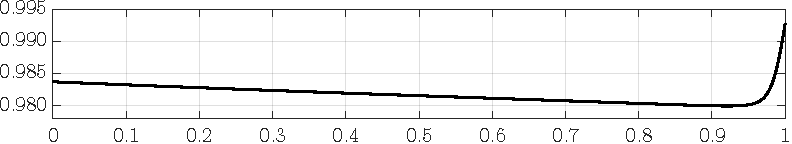
\includegraphics[width=0.7\columnwidth]{./responses-rev-1/stability-cntrl-2.pdf}
\caption{The spectral radius of the mean-square stability verification matrix, $\rho(\mathit{\Lambda})$, as a function of the dropout compensation factor $\mathit{\Phi}$ for the rotary inverted pendulum under the proposed infinite-horizon linear–quadratic regulation (LQR) [4—Fig. 12]}\label{fig:stability-coeff}
\end{center}
\end{figure}
\begin{figure}[h!]
\begin{center}
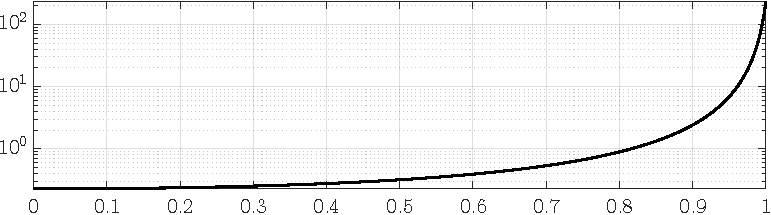
\includegraphics[width=0.7\columnwidth]{./responses-rev-1/cost-cntrl-2.pdf}
\caption{Long-run average cost $J_{\infty}^{\star}(\mathit{\Phi})$ for the rotary inverted pendulum under the proposed infinite-horizon LQR for $\Sigma_{w}=4\cdot 10^{-6} I_4$. See [4—Fig. 13] for similar results, obtained with $\Sigma_{w}=2.5\cdot 10^{-9} I_4$.}\label{fig:cost-coeff}
\end{center}
\end{figure}
\begin{figure}[h!]
\begin{center}
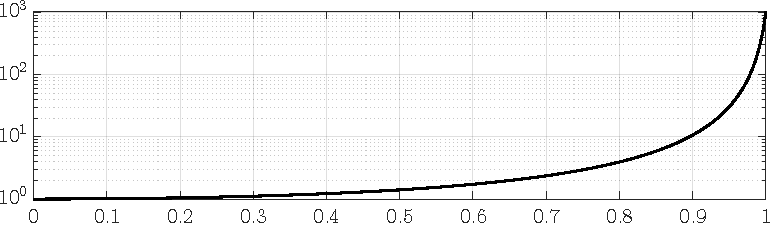
\includegraphics[width=0.7\columnwidth]{./responses-rev-1/cost-ratio-2.pdf}
\caption{The ratio $\frac{J_{\infty}^{\star}(\mathit{\Phi})}{J_{\infty}^{\star}(\mathit{0})}$ for the rotary inverted pendulum with $\Sigma_{w}=4\cdot 10^{-6} I_4$.}\label{fig:cost-ratio}
\end{center}
\end{figure}\\[-4mm]
Figure \ref{fig:stability-coeff} shows that the values of $\rho(\Lambda)$ decrease from $0.9837$ in $0$ to $0.9799$ in $0.921$ and then monotonically increase to $0.9928$ in $1$. This indicates that $\mathit{\Phi} = 0.921$ provides the most stable closed-loop behavior in the mean-square sense. The value of $\rho(\Lambda)<1$ indicates the convergence rate of the closed-loop system to the mean-square stable steady state, as discussed in the response to Comment 3 of Reviewer 16. Therefore, the lower values of $\rho(\Lambda)$ are desirable, and $\mathit{\Phi} = 0.1$ produces $\rho(\Lambda)=0.9832$, which is slightly lower than $0.9837$, obtained for $\mathit{\Phi} = 0$. Furthermore, all admissible values of $\mathit{\Phi}$ produce mean-square stable system behavior, though with different long-run average costs.\\
The long-run average cost $J_{\infty}^{\star}$ for $\Sigma_{w}=4\cdot 10^{-6} I_4$ in Figure \ref{fig:cost-coeff} increases monotonically in $\mathit{\Phi}$, passing from $0.22654$ in $0$ to $0.22923$ in $0.1$, $0.23715$ in $0.2$, $0.25193$ in $0.3$, $0.27676$ in $0.4$,
$0.31823$ in $0.5$, $0.39114$ in $0.6$, $0.53508$ in $0.7$, $0.89246$ in $0.8$, 
$2.41235$ in $0.9$, and $232.55649$ in $1$. Similar results are shown in [4] in Figure 13 for $\Sigma_{w}=2.5\cdot 10^{-9} I_4$. \\
Figure \ref{fig:cost-ratio} presents the ratio of long-run average cost $J_{\infty}^{\star}$ in $\mathit{\Phi}$ to $J_{\infty}^{\star}$ in $0$, indicating an increase of three orders of magnitude in the cost for $\mathit{\Phi}=1$ compared to $\mathit{\Phi}=0$. For $\mathit{\Phi}=0.1$, the long-run average cost $J_{\infty}^{\star}$ is close to the cost in $\mathit{\Phi}=0$. \\
The long-run average cost and mean-square stability analyses in [4] reveal that the dropout compensation factors, ranging from $0$ to $0.921$, provide a trade-off between the two metrics, with particular choices depending on the design's priorities. The choice of $\mathit{\Phi} = 0.1$ presents a compelling alternative to the zero-input message dropout compensation (MDC) strategy ($\mathit{\Phi} = 0$) by offering a slightly higher cost but faster convergence to the steady state. The hold-input MDC ($\mathit{\Phi} = I$) yields mean-square stable closed-loop system behavior at a significantly higher cost. \\
The analysis above refers to the baseline case of no future control inputs and perfect CSI. The results of this letter enable analyses under imperfect CSI and a hybrid MDC that combines the transmission of multiple control inputs with the scaling of inputs to actuators when necessary. Although the space constrains of an L-CSS letter prevent us from discussing the effects of different scaling factors $\mathit{\Phi}$, we present the spectral radius of the mean-square stability verification matrix $\rho(\mathit{\Lambda})$ and the long-run average cost $J_{\infty}^{\star}$ as a function of the number of future controls $n_f$ for the three most significant values of the dropout compensation factor $\mathit{\Phi}$ ($0$, $0.921$, and $1$ from the baseline case), in addition to the case of $\mathit{\Phi}=0.1$, in the figures below.
\begin{figure}[h!]
\begin{center}
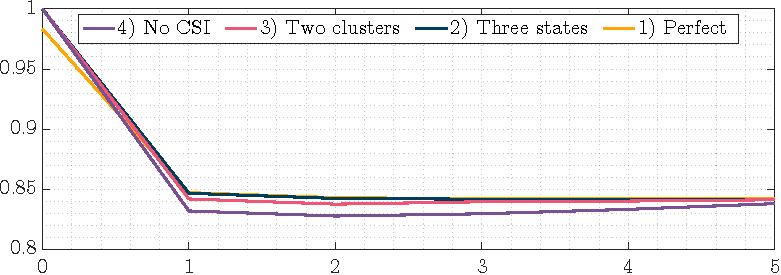
\includegraphics[width=0.8\columnwidth]{./responses-rev-1/stability-cntrl-a.pdf}
\caption{The spectral radius of the mean-square stability verification matrix, $\rho(\mathit{\Lambda})$, as a function of the number of control inputs $n_f$ for the rotary inverted pendulum under the proposed infinite-horizon linear–quadratic regulation (LQR) with the dropout compensation factor $\mathit{\Phi}=0.1$—Fig. 2 in the revised version of the letter}\label{fig:stability-coeff-a}
\end{center}
\end{figure}
\begin{figure}[h!]
\begin{center}
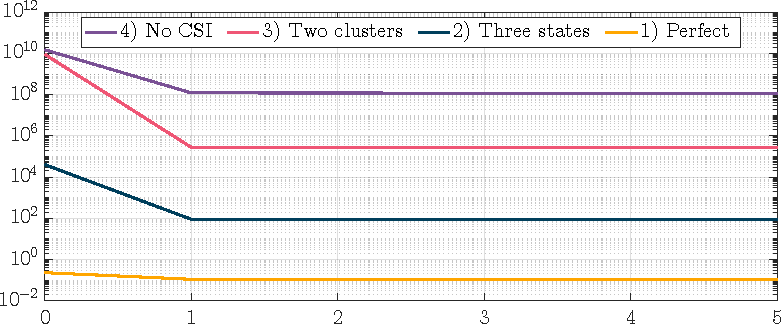
\includegraphics[width=0.8\columnwidth]{./responses-rev-1/cost-cntrl-a.pdf}
\caption{The long-run average cost, $J_{\infty}^{\star}$, as a function of the number of control inputs $n_f$ for the rotary inverted pendulum under the proposed infinite-horizon linear–quadratic regulation (LQR) with the dropout compensation factor $\mathit{\Phi}=0.1$—Fig. 3 in the revised version of the letter}\label{fig:cost-cntrl-a}
\end{center}
\end{figure}
\begin{figure}[h!]
\begin{center}
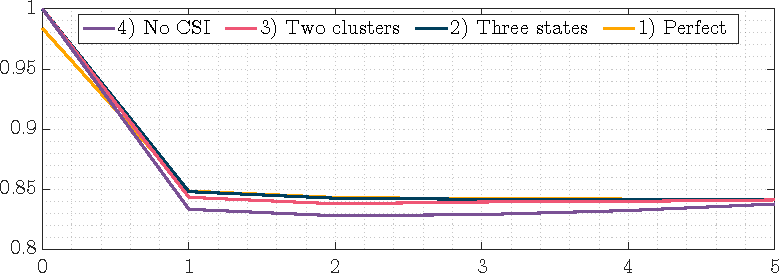
\includegraphics[width=0.8\columnwidth]{./responses-rev-1/stability-cntrl-0.pdf}
\caption{The spectral radius of the mean-square stability verification matrix, $\rho(\mathit{\Lambda})$, as a function of the number of control inputs $n_f$ for the rotary inverted pendulum under the proposed infinite-horizon linear–quadratic regulation (LQR) with the dropout compensation factor $\mathit{\Phi}=0$}\label{fig:stability-coeff-0}
\end{center}
\end{figure}
\begin{figure}[h!]
\begin{center}
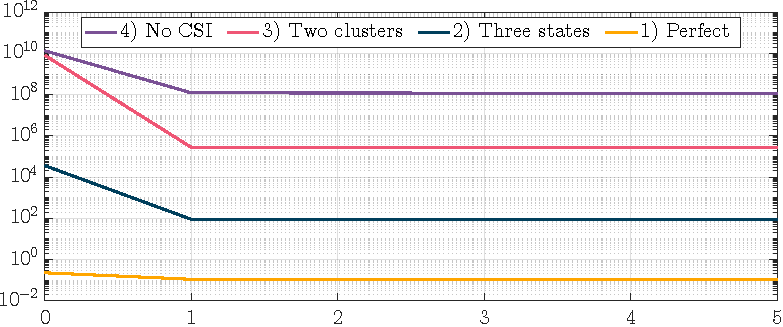
\includegraphics[width=0.8\columnwidth]{./responses-rev-1/cost-cntrl-0.pdf}
\caption{The long-run average cost, $J_{\infty}^{\star}$, as a function of the number of control inputs $n_f$ for the rotary inverted pendulum under the proposed infinite-horizon linear–quadratic regulation (LQR) with the dropout compensation factor $\mathit{\Phi}=0$}\label{fig:cost-cntrl-0}
\end{center}
\end{figure}
\begin{figure}[h!]
\begin{center}
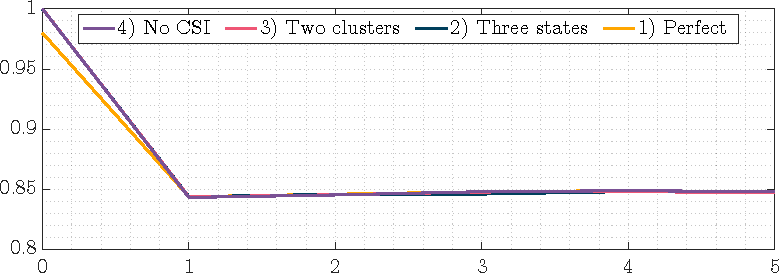
\includegraphics[width=0.8\columnwidth]{./responses-rev-1/stability-cntrl-9.pdf}
\caption{The spectral radius of the mean-square stability verification matrix, $\rho(\mathit{\Lambda})$, as a function of the number of control inputs $n_f$ for the rotary inverted pendulum under the proposed infinite-horizon linear–quadratic regulation (LQR) with the dropout compensation factor $\mathit{\Phi}=0.921$}\label{fig:stability-coeff-9}
\end{center}
\end{figure}
\begin{figure}[h!]
\begin{center}
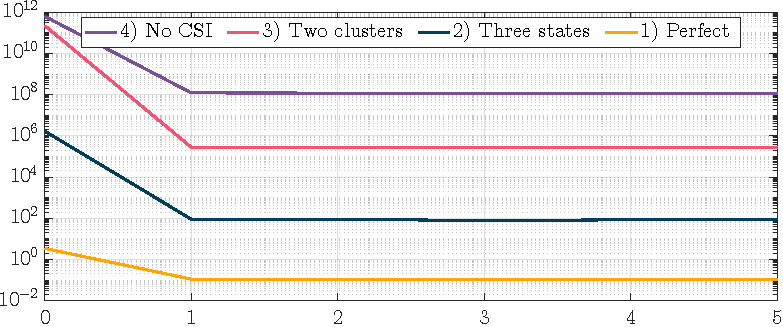
\includegraphics[width=0.8\columnwidth]{./responses-rev-1/cost-cntrl-9.pdf}
\caption{The long-run average cost, $J_{\infty}^{\star}$, as a function of the number of control inputs $n_f$ for the rotary inverted pendulum under the proposed infinite-horizon linear–quadratic regulation (LQR) with the dropout compensation factor $\mathit{\Phi}=0.921$}\label{fig:cost-cntrl-9}
\end{center}
\end{figure}
\begin{figure}[h!]
\begin{center}
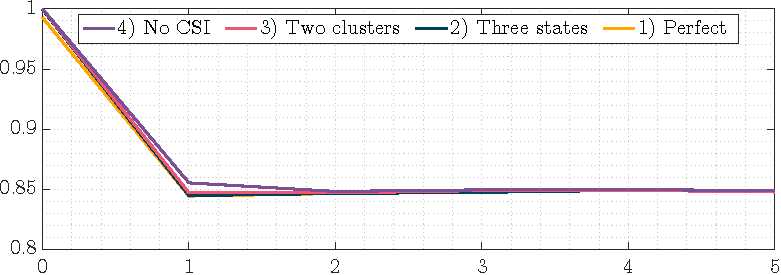
\includegraphics[width=0.8\columnwidth]{./responses-rev-1/stability-cntrl-1.pdf}
\caption{The spectral radius of the mean-square stability verification matrix, $\rho(\mathit{\Lambda})$, as a function of the number of control inputs $n_f$ for the rotary inverted pendulum under the proposed infinite-horizon linear–quadratic regulation (LQR) with the dropout compensation factor $\mathit{\Phi}=1$}\label{fig:stability-coeff-1}
\end{center}
\end{figure}
\begin{figure}[h!]
\begin{center}
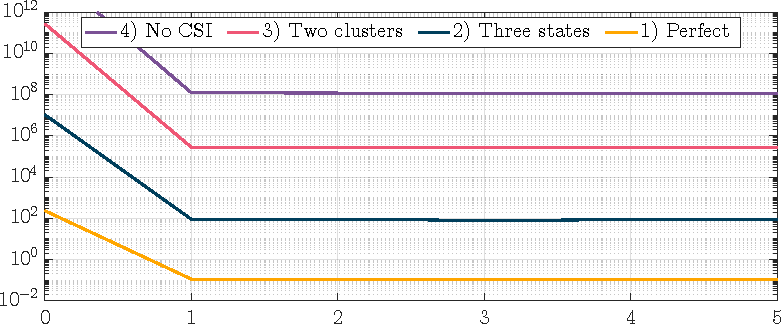
\includegraphics[width=0.8\columnwidth]{./responses-rev-1/cost-cntrl-1.pdf}
\caption{The long-run average cost, $J_{\infty}^{\star}$, as a function of the number of control inputs $n_f$ for the rotary inverted pendulum under the proposed infinite-horizon linear–quadratic regulation (LQR) with the dropout compensation factor $\mathit{\Phi}=1$}\label{fig:cost-cntrl-1}
\end{center}
\end{figure}\\
}
\textcolor{black}{Figures \ref{fig:stability-coeff-a} and \ref{fig:cost-cntrl-a} correspond to Figures 2 and 3 in the revised version of the letter. By comparing Figure \ref{fig:stability-coeff-a} to Figure \ref{fig:stability-coeff-0} and Figure \ref{fig:cost-cntrl-a} to Figure \ref{fig:cost-cntrl-0}, we observe that differences between the closed-loop system characteristics under the MDC factors $\mathit{\Phi}$ of $0$ and $0.1$ are marginal. Our choice to present the case of $\mathit{\Phi}=0.1$ is motivated by its generality, as the zero-input MDC ($\mathit{\Phi}=0$) is a very special case that requires less complex analysis. The closed-loop system with $\mathit{\Phi}=0.1$ has slightly better performance in terms of stability at the price of a slightly worse long-run average cost.\\
Similar to the baseline case, Figures \ref{fig:stability-coeff-a}–\ref{fig:cost-cntrl-1} show that the MDC factor $\mathit{\Phi}=0.921$ yields the most stable closed-loop system for all considered numbers of control inputs, $n_f$, at significantly higher long-run average costs (Figures \ref{fig:stability-coeff-9} and \ref{fig:cost-cntrl-9}). The hold-input MDC strategy ($\mathit{\Phi}=1$) ensures stable closed-loop system behavior; however, it has the lowest convergence rate and the highest long-run average cost, making it less desirable in terms of performance (Figures \ref{fig:stability-coeff-1} and \ref{fig:cost-cntrl-1}).} \\[4mm]
%%%
\textbf{Reviewer 9—Questions on notations—1)}\textit{ %
What is the difference between $u^{n_f}_T$ in Eq. (15) and $\bar{u}$ in Eq (10). What is the definition on $f$ in Eq (15). It is a little bit mess in notations. I suggest you to check it through all letter.}\\[2mm]
\textbf{Authors' response on parameter tuning question 1:} \textcolor{black}{We thank the Reviewer for the question. Equation (15) is a part of a sentence stating that ``$\bm{u}_{T}^{n_f}$ is a sequence of length $T$ of control messages as in (10) such that $\bar{u}_{(k+f\mid k)} = K_{(k+f,\hat{\theta}_{k-1})}x_k$.'' This statement means that (15) provides a constraint for a generic control message $\hat{u}_k$ defined by (10), where $\hat{u}_k = \left([\bar{u}_{(k+f\mid k)}^{\top}]_{f=0}^{n_f}\right)^{\!\top}$. 
The meaning of $f$ becomes self-explanatory from substituting the generic elements $\bar{u}_{(k+f\mid k)}$ of the control message $\hat{u}_k$ in (10) with their specific definition in (15):
$\hat{u}_k = \left([(K_{(k+f,\hat{\theta}_{k-1})}x_k)^{\top}]_{f=0}^{n_f}\right)^{\!\top}$. In words, $f$ indexes the elements of the control message, % at time $k$, 
with $f=0$ indicating the current input, and $f\geq 1$ pinpointing specific future inputs. The meaning of $f$ never changes throughout this letter, and the notation is consistent. 
$f \in \mathbb{Z}^{0+}$ and $f\leq n_f$ in (10), (22), and (39). Finally, this letter uses parenthesis to identify sequences. Thus, $\bm{u}_{T}^{n_f}$ can be expressed as $\bm{u}_{T}^{n_f} = (\hat{u}_k)_{k=0}^{T-1}$, where $\hat{u}_k$ is defined by (10) and each element of $\hat{u}_k$ satisfies (15). 
}\\[4mm]
%%%
\textbf{Reviewer 9—Questions on notations—2)}\textit{ %
Where is the definition of $\mathbb{B}$ in Eq. (29)?}\\[2mm]
\textbf{Authors' response on parameter tuning question 2:} \textcolor{black}{We thank the Reviewer for the question. If the Reviewer refers to $\mathcal{B}$, it is defined by equation (31), which is shown at the top of page 5, as indicated by the sentence that follows equation (29). There is no $\mathbb{B}$ in this letter.}\\[4mm]
%%%
\textbf{Reviewer 9—Other suggestion on expression—1)}\textit{ %
Abbreviation of linear–quadratic regulators (LQR) should be added for highlight in introduction.}\\[2mm]
\textbf{Authors' response to the first suggestion on expression:} \textcolor{black}{
We thank the Reviewer for the suggestion. In the introduction, we refrain from using the abbreviation LQR for linear–quadratic regulators to avoid confusing it with different, albeit related, meanings, as we utilize LQR to refer specifically to linear–quadratic regulation in Section 3 and beyond.}\\[4mm]
%%%
\textbf{Reviewer 9—Other suggestion on expression—2)}\textit{ %
The sequences in Eq. (14) are suggested to expressed as $[x_t]^k_{t=0}$, instead of $(x_t)^k_{t=0}$ for example.}\\[2mm]
\textbf{Authors' response to the second suggestion on expression:} \textcolor{black}{We thank the Reviewer for the suggestion. This letter follows the notation of [4], % \cite{yZL-2025-automatica}, 
where curly brackets enclose the values of sets, square brackets define matrices, and parentheses identify sequences. Thus, we refrain from using square brackets to define sequences to avoid confusion between sequences and matrices.}\\[4mm]
%%%
\textbf{Authors' concluding remark:} \textcolor{black}{We are grateful to the Reviewer for the comments and suggestions. We sincerely hope the above explanations have adequately addressed the Reviewer's concerns.}
% \putbib
% \end{bibunit}